\documentclass[french,xcolor=dvipsnames]{beamer}
\usepackage[utf8]{inputenc}
\usepackage[T1]{fontenc}
\usepackage{amsmath}
\usepackage{amsfonts}
\usepackage{amssymb}
\usepackage{graphicx}
\usetheme{Antibes}
\usepackage{wrapfig}
\usepackage{tikz}
\usecolortheme[named=Maroon]{structure}
\graphicspath{{Images/}}

\begin{document}
	\title{Hexaflexagones}
	\subtitle{Construction et propriétés}
	%\subtitle{Constructions et propriétés}
	%\logo{}
	%\institute{}
	%\date{}
	%\subject{Courbes de largeur constantes}
	%\setbeamercovered{transparent}
	%\setbeamertemplate{navigation symbols}{}
	\frame[plain]{\maketitle}
	

\AtBeginSection
{
\frame{{Plan}\tableofcontents[currentsection]}
}

	\frame{{Plan}\tableofcontents}
	
	\section{Introduction}
		\subsection{(bref) Historique}
		\begin{frame}{Un bref historique}

			\begin{list}{Intro}{}
				\item[$\textit{1939}$.] Découverte  par Arthur Stone
				\item[$\textit{1956}$.]Colonne de Martin Gardner dans \textit{Scientific American}
				\item[Polulaire mais pas de succèes commercial]
			\end{list}
		\end{frame}
		
		\subsection{Démonstration/Mise en évidence}
		\begin{frame}{(Démonstration)}
			METTRE 3 4 PHOTOS DE FLEXAGONES POUR MONTRER CE QU'IL SE PASSE\\
			IL FAUDRA BIEN SÛR PLUSIEURS FRAME !!!!!!
		\end{frame}
		\begin{frame}{(Démonstration)}
			METTRE 3 4 PHOTOS DE FLEXAGONES POUR MONTRER CE QU'IL SE PASSE\\
			IL FAUDRA BIEN SÛR PLUSIEURS FRAME !!!!!!
		\end{frame}
		\begin{frame}{(Démonstration)}
			METTRE 3 4 PHOTOS DE FLEXAGONES POUR MONTRER CE QU'IL SE PASSE\\
			IL FAUDRA BIEN SÛR PLUSIEURS FRAME !!!!!!
		\end{frame}
		\begin{frame}{(Démonstration)}
			METTRE 3 4 PHOTOS DE FLEXAGONES POUR MONTRER CE QU'IL SE PASSE\\
			IL FAUDRA BIEN SÛR PLUSIEURS FRAME !!!!!!
		\end{frame}
		\begin{frame}{(Démonstration)}
			METTRE 3 4 PHOTOS DE FLEXAGONES POUR MONTRER CE QU'IL SE PASSE\\
			IL FAUDRA BIEN SÛR PLUSIEURS FRAME !!!!!!
		\end{frame}
		
		\begin{frame}{Ajout de faces}
		IL FAUT MONTRER QU'ON PEUT AJOUTER DES FACES ET QUE C'EST COOL !!
		\end{frame}
		
		\subsection{Objectifs}
		\begin{frame}{Objectifs}
			Programmer un logiciel donnant les patrons d'hexaflexagones
		\end{frame}
		
		
	\section{Préliminaire}
	
		\subsection{Représentations}
		
		\subsubsection{Patrons}
		\begin{frame}{Patrons}
			\begin{figure}
				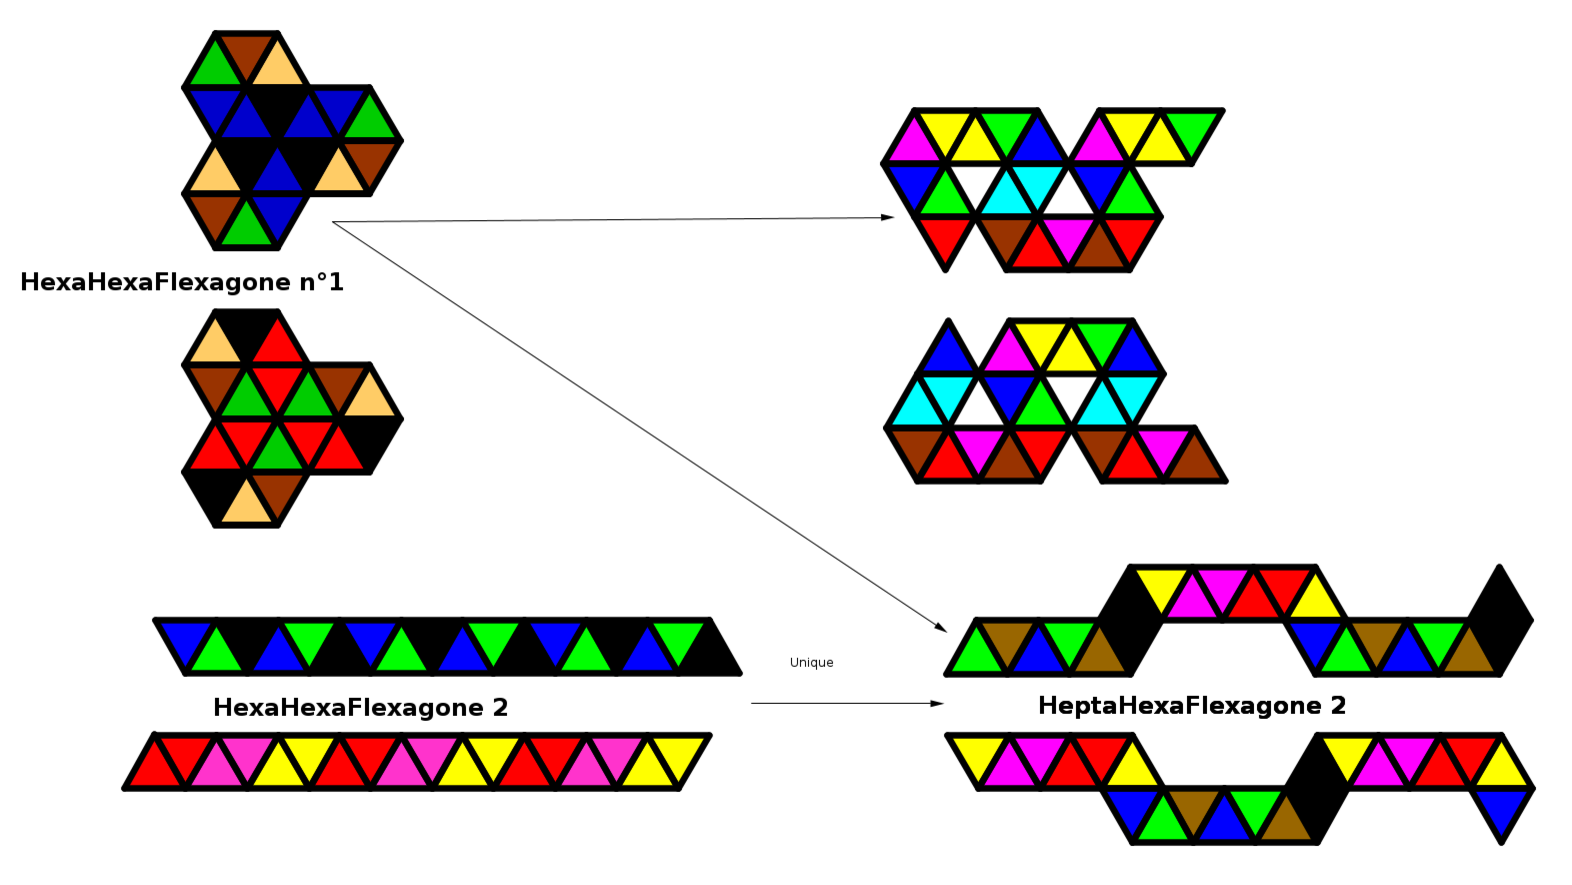
\includegraphics[scale=0.19]{exemples_patrons.png}
			\end{figure}
		\end{frame}
		
		\begin{frame}{Problèmes}
			PRATIQUE NI POUR LA THEORIE NI A REPRESENTER EN MACHINE A PRIORI\\
			C'est pourtant ce qu'on cherche à construire.
		\end{frame}
				
		\subsubsection{Graphes}
		\begin{frame}{Tuckerman Traverse}
			\begin{figure}
				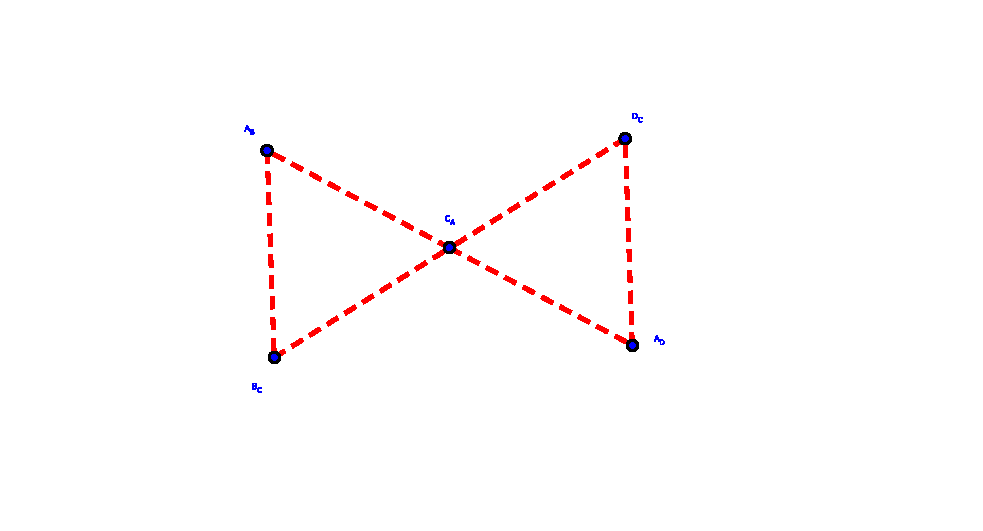
\includegraphics[scale=0.6]{TT_graphe_4.eps}
				\caption{Tuckerman Traverse du 4-hexaflexagon}
			\end{figure}
		\end{frame}		
		
		\begin{frame}{Triangulations}
			TRIANGULATIONS ICI C GENIAL		
		\end{frame}
		
		\subsection{Dénombrement}
		\begin{frame}{Nombres de Catalan}
			METTRE UN IMAGE POUR JUSTIFIER LES NOMBRES DE CATALAN SUR LES TRIANGULATIONS DE POLYGONES ET PUIS VOILÀ
		\end{frame}
		\begin{frame}{Groupe diédral}
			GROUPE DIÉDRAL POUR LES TRIANGULATIONS
		\end{frame}
		
		\begin{frame}{Action de groupe}
			\begin{definition}
			Pour un ensemble X, un groupe G défini naturellement la relation d'équivalence sur X par
			\[
				\forall x,y \in x, x \equiv y \Leftrightarrow \exists g \in G, x=g.y
			\]
			\end{definition}
			
			On étudie $T_{n}$ sous l'action de $D_{n}$.
		\end{frame}
		\begin{frame}{Lemme de Burnside}
			\begin{theorem}{\underline{Lemme de Burnside} \small{(dû à Cauchy puis Frobenius)}\\}
				G un groupe, X un ensemble fini, alors
				\[
				\mid X/G \mid = \sum_{g\in G}{\mid Fix(g) \mid}
				\]
				où $\mid X/G \mid$ est le quotient de $X$ sous l'action de $G$ et \\s$Fix(g) = \{x\in X, g.x = x\}$ est l'ensemble des éléments de X invariants par g.
			\end{theorem}
		\end{frame}
		
		\begin{frame}{Application au dénombrement}
			MONTRER ASSEZ VITE COMMENT LES ROTATIONS FONCTIONNENT (CENTRE DU POLYGONE) ET PASSER SUR LES SYMÉTRIES (SANS DOUTE TROP LONG)
		\end{frame}
		
		\begin{frame}{Finalement}
		On a compté nos flexagones
		{\Large
		\[
			\mid F_{n} \mid = \frac{1}{n}C_{n-2} + \frac{1}{2}C_{\frac{n}{2}-1} + \frac{2}{3}C_{\frac{n}{3}-1}
		\]
		}
		\end{frame}		
		
		
	\section{En machine}
		\subsection{Représentation}
			
		\begin{frame}{Polygones}
			\begin{description}
			\item[*]Un entier: l'ordre du polygone
			\item[*]Une liste de couples: les arêtes internes
			\end{description}
			
			\begin{figure}
				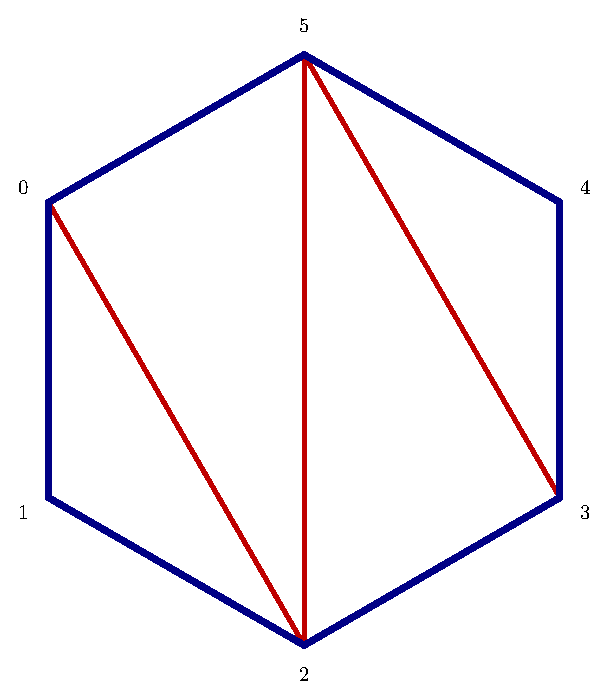
\includegraphics[scale=1]{exemple_6_rot.ps}
			\end{figure}
		\end{frame}
\end{document}
